\FloatBarrier
\section{آشنایی با فرمت های ذخیره سازی}\label{ch:background|sec:format-storage}

داده‌های \mri نیز مانند دادگان دیگر در سایر زمینه ها نیاز است که در یک فرمت واحد ذخیره شود که مستقل از ارائه دهنده و یا فروشنده آن اطلاعات باشد. این فرمت ذخیره سازی منظم، به محققان این اجازه را می‌دهد که به ساده‌ترین شکل ممکن داده‌ خود را عوض کنند.
فرمت داده خاص منظم‌شده 
\LTRfootnote{Descipline-Specific data format}
به دانشمندان و محققان کمک می‌کند تااز محدودیت هایی که از طرف فروشندگان خاص آن داده یا تکنولوژی های اختصاصی، تحمیل می‌شود، فرار کنند.

تصویربرداری پزشکی، استانداردی مانند\textit{ تصویر برداری دیجیتال و ارتباطات در پزشکی}
\LTRfootnote{Digital Imaging and COmmunication in Medicine}(\lr{DICOM})
دارد که به گروه رادیولوژی اجازه این را می‌دهد که داده های فروشندگان مختلف را در یک فرمت واحد ذخیره کنند.
زیرشاخه‌ی تصویربرداری عصبی نیز فرمت مخصوص خود یعنی \textit{طرح فناوری اطلاعات انفورماتیک عصبی}
\LTRfootnote{Neuroimaging Informatics Technology Initiative}(\lr{NIfTI})
را دارند که پروژه های وسیعی با آن فرمت ها انجام شده است.
اما این فرمت ها برای استفاده از عملیات بازسازی تصویر زیاد مناسب نیستند چرا که اطلاعات علمی که الگوریتم های
بازسازی با آن‌ها کار می‌کنند را شامل نمی‌شوند.
برای کارکردن با فرمت خام بازسازی، فرمت \textit{داده خام \lr{ISMRM}}
\LTRfootnote{ISMRM Raw Data format}(\lr{ISMRMRD})
پیشنهاد شده است که مفصلا در مورد آن صحبت خواهد شد.




\subsection{فرمت ذخیره سازی\lr{ISMRMRD}}

\textit{انجمن بین‌المللی تشدید مغناطیسی در پزشکی}
\LTRfootnote{International Society for Magnetic Resonance in Medicine}(\lr{ISMRM})
یک انجمن غیرانتفاعی است که نظم در زمینه های توسعه و نوآوری و کاربرد های تشدید مغناطیسی فعالیت‌هایی را در سطح جهانی ترویج می‌دهد.
\cite{wiki:International_Society_for_Magnetic_Resonance_in_Medicine}
استاندارد \lr{ISMRMRD}
توسط یک زیرکمیته از \lr{ISMRM} در سال 2013 توسعه می‌یابد.

فرمت خامی که این انجمن معرفی کرده است مخصوص داده های خام \mri پیش از هرگونه عملیات بازسازی، پدینگ صفر
\LTRfootnote{Zero padding}
، درون‌یابی، فیلتر کردن و یا تبدیل فوریه گرفتن، می‌باشد. ایت فرمت طراحی شده است تا اطلاعات مربوط به بازسازی را مستقل از فروشندگان مختلف \mri در اختیار محققان قرار دهد چرا که تا پیش از آن هریک از آن فروشندگان فرمت اختصاصی خود را داشته اند. همچنین ابزار هایی جهت تبدیل داده های فروشندگان مختلف را به این فرمت در گیت هاب خود ارایه داده اند. از این فرمت می‌توان در زبان های برنامه نویسی متلب، پایتون و سی پلاس پلاس استفاده کرد. 
\cite{ISMRM}

\begin{figure}[t!]
	\centering
	\copyrightbox[b]{
		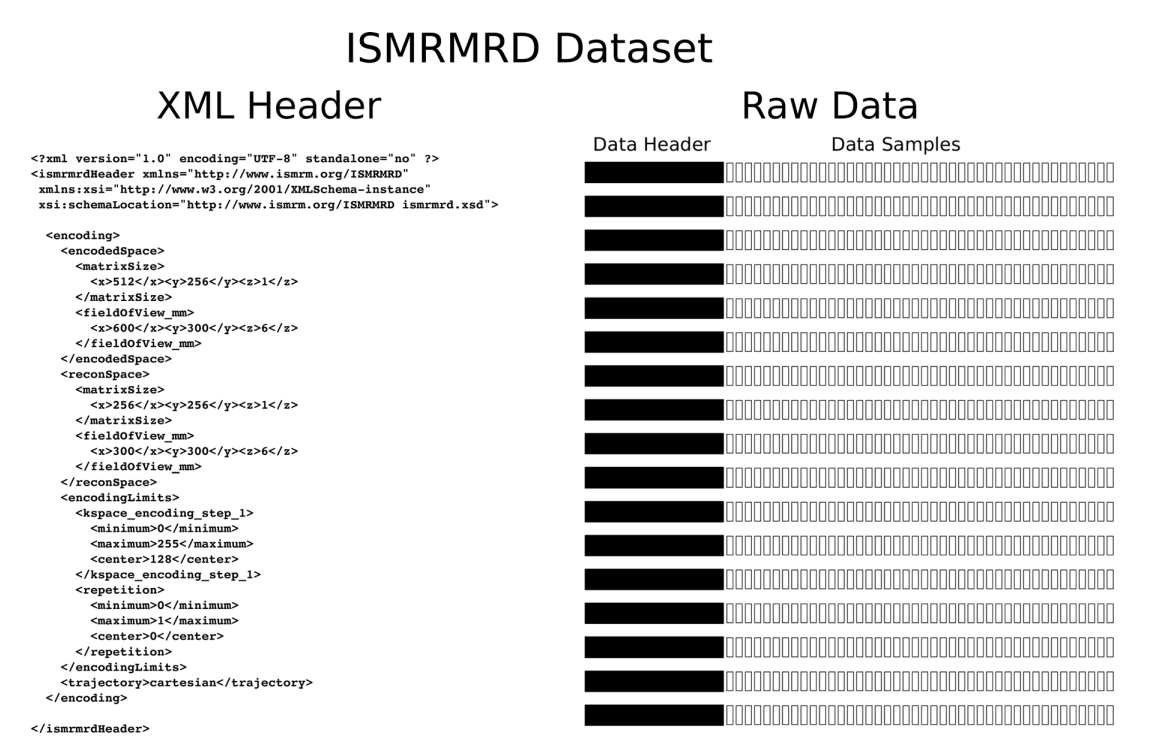
\includegraphics[width=0.85\linewidth]{chapters/chapter-2/figs/ismrmrd-dataset}
	}{\doiSource{10.1002/mrm.26089}}
	\removevspace[1]
	\caption{دیتاست فرمت \lr{ISMRMRD}}
	\label{fig:ismrmrd-dataset}
\end{figure}

دیتاست ارایه شده در شکل \ref{fig:ismrmrd-dataset} از دو قسمت اصلی تشکیل شده است:

\removevspace[1]
\begin{itemize}
	\item 
	یک هدر \lr{XML}.
	\item 
	داده ی خام.
\end{itemize}

\begin{figure}[t!]
	\centering
	\copyrightbox[b]{
		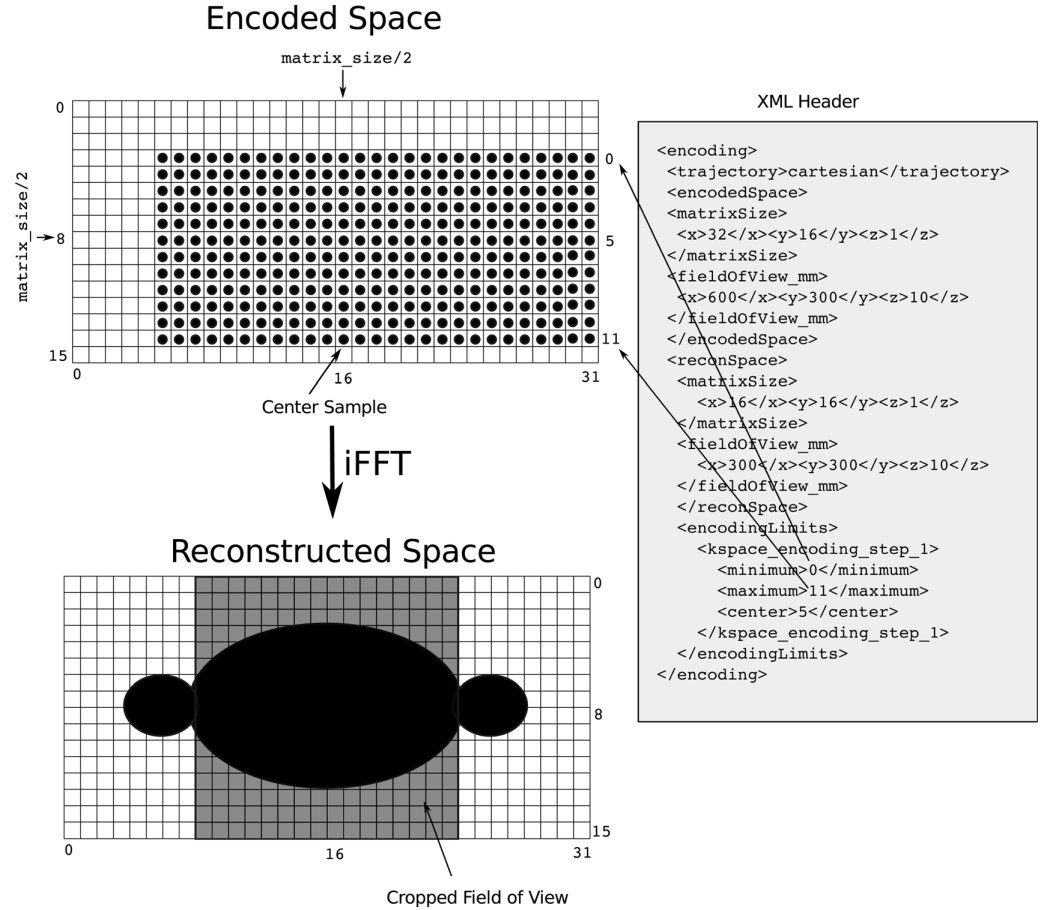
\includegraphics[width=0.7\linewidth]{chapters/chapter-2/figs/ismrmrd-encodedSpace}
	}{\doiSource{10.1002/mrm.26089}}
	\caption{}
	\label{fig:ismrmrd-encodedspace}
\end{figure}




\begin{table}[b!]
	\begin{latin}\footnotesize
	\begin{tabularx}{\linewidth}{lXXXX}
	\hline
	ISMRMRD & Bruker & GE & Philips & Siemens \\ \hline
	kspace\_encode\_step\_1 & encode step 1 &‌ Frame&‌ e1 & Line\\
	kspace\_encode\_step\_2 & encode step 2 &‌ – &‌ e2 &‌ Partition\\
	Average & – & – &  Measurement & Acquisition\\
	Slice & Slice‌&  Slice &  Location & Slice \\
	Contrast &‌ Echo &‌ Echo & Echo & Echo\\
	Phase &‌ ‌– &‌ – &‌ Cardiac phase & Phase\\
	Repetition & Repetition &‌ Repetition&‌ Dynamic scan& Repetition\\
	Set & – & – &‌Row& Set\\
	Segment & – & – & – & Segment\\ \hline
	\end{tabularx}
	\end{latin}
\caption{}
\end{table}

